\documentclass[12pt,a4paper]{article}
\usepackage[utf8]{inputenc}
\usepackage[russian]{babel}
\usepackage[OT1]{fontenc}
\usepackage{amsmath}
\usepackage{amsfonts}
\usepackage{amssymb}
\usepackage{graphicx}
\graphicspath{{Images/}}
\usepackage[left=2cm,right=2cm,top=2cm,bottom=2cm]{geometry}
\usepackage{calc}
\usepackage{wrapfig}
\usepackage{setspace}
\usepackage{indentfirst}
\usepackage{subfigure}
\usepackage{multirow}


\title{
Отчет о выполнении лабораторной работы 2.1.4 

Определение теплоемкости твердых тел
}

\author{Варламов Антоний, группа Б02-928}

\begin{document}

\maketitle

\newpage

\section{Теоретический материал}

	В данной работе происходит измерение теплоемкости твердого тела с использованием следующей принципиальной связи:
	
	\begin{equation}
		C = \frac{\Delta Q}{\Delta T}
		\label{eq:first_eq_of_thermal_capacity}
	\end{equation}
	
	Определение количества теплоты, переданного телу вызывает некоторые затруднения, так как часть теплоты будет передано окружающей среде через стенки калориметра. В итоге, количество теплоты, переданное телу с учетом теплопотерь через стенки можно определить как:
	
	\begin{equation}
		\Delta Q = P\Delta t - \lambda \left( T - T_{\text{к}} \right) \Delta t,
		\label{eq:termal_with_heat_lossing}
	\end{equation}
	 где $P$ -- мощность нагревателя, $\lambda$ -- коэффициент теплоотдачи стенок калориметра, $T$ -- температура тела, $T_{\text{к}}$ -- температура окружающего калориметр воздуха, $\Delta t$ -- время, в течении которого происходит нагрев.
	 
	 Из уравнений (\ref{eq:first_eq_of_thermal_capacity}) и (\ref{eq:second_eq_of_thremal_capacity}) получаем:
	 
	 \begin{equation}
	 	C = \frac{P - \lambda \left(T - T_{\text{к}} \right) }{\Delta T /\Delta t}
	 	\label{eq:second_eq_of_thremal_capacity}
	 \end{equation}
	 
	Формула (\ref{eq:second_eq_of_thremal_capacity}) является основной расчетной формулой данной работы.
	
	В формуле (\ref{eq:second_eq_of_thremal_capacity} в знаменателе стоит величина, для определения которой воспользуемся следующей методикой:
	
	Построим график зависимости $\frac{\Delta T}{\Delta t} = f \left( T \right)$ для широкого диапазона температур, после чего экстраполируем его для значения $T = T_{\text{к}}$. В таком случае формула (\ref{eq:second_eq_of_thremal_capacity}) приобретает вид:
	
	\begin{equation}
		C = \frac{P}{\left( \Delta T / \Delta t \right)_{T_{\text{к}}}}
		\label{eq:final_eq_for_capacity}
	\end{equation}
	
	Измерение температуры строится на принципе линейной зависимости сопротивления материала от изменения температуры по закону:
	
	\begin{equation}
		R_{T} = R_{0} \left( 1 + \alpha \Delta T \right),
	\end{equation}
	
	Где $R_{0}$ -- сопротивление термометра при комнатной температуры, $R_{T}$ -- сопротивление термометра при данной температуре. Учитывая данную зависимость, получаем итоговый вид для основной формулы:
	
	\begin{equation}
		C = \frac{PR\alpha}{\left( \frac{dR}{dt} \right)_{T_{\text{к}}}\left( 1 + \alpha \Delta T_{\text{К}} \right)}
		\label{eq:capacity}
	\end{equation}	 
	
	Коэффициент $\alpha$, входящий в данную формулу для меди равен $\alpha = 4,28 \cdot 10^{-3} \, K^{-1}$, все остальные величины определяются экспериментально.
	
	\newpage

\section{Схема установки}
	
	\begin{wrapfigure}[9]{r}{0.3\textwidth}
		\vspace{-2.5ex}
		\begin{center}
			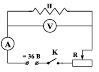
\includegraphics[width = 0.2\textwidth]{schem_of_facility}
			\caption{Схема установки}
			\label{fig:schem_of_facility}
		\end{center}
	\end{wrapfigure}
	
	Установка состоит из калориметра с пенопластовой изоляцией, помещенного в ящик из многослойной клееной фанеры. Внутренние стенки калориметра выполнены из материала с высокой теплопроводностью. Надежность теплового контакта между телом и стенками обеспечивается их формой: они имеют форму усеченных конусов и плотно прилегают друг к другу. Для выталкивания образца служит винт в донышке внутренней стенки калориметра.
	
	В стенку калориметра вмонтированы электронагреватель и термометр сопротивления. Схема включения нагревателя изображена на рисунке (\ref{fig:schem_of_facility}). Система реостатов позволяет установить нужную силу тока в цепи нагревателя. По амперметру и вольтметру определяется мощность, выделяемая током в нагревателе. Величина сопротивления термометра нагревателя  измеряется мостом постоянного тока.
	
	\begin{figure}[h!]
		\begin{center}
			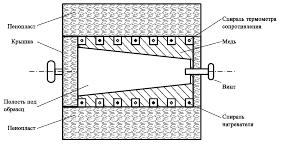
\includegraphics[width = 0.5\textwidth]{Ris_of_facility}
			\caption{Устройство калориметра}
			\label{fig:Ris_of_facility}
		\end{center}
	\end{figure}	
	
	На рисунке (\ref{fig:Ris_of_facility}) изображено устройство калориметра.
	
	Запишем также иные параметры экспериментальной установки (Данные занесем в таблицу \ref{tab:results_of_measuring_of_depence_resistance_for_time}):
	
	\begin{table}[h!]
		\centering
		\begin{tabular}{|c|c|c|c|}
			\hline
			материал образца: & железо          & латунь          & алюминий        \\ \hline
			масса образца, г  & $815,1 \pm 0,1$ & $875,5 \pm 0,1$ & $294,2 \pm 0,1$ \\ \hline
		\end{tabular}
		\caption{Параметры исследуемых образцов}
		\label{tab:param_of_facility}
	\end{table}
	
	$$R_{0} = 18,105 \pm 0,01 \, \text{Ом}, \quad t_{0} = 23^{\circ} \pm 1 ^{\circ} C$$
	
	$$ U = 36 \, \text{В}, \, I = 0,6 \, \text{А}, \, P = 10,8 \, \text{Вт} $$
	
	
	



	\newpage

\section{Выполнение работы}

Снимем зависимость R(t) для калориметра, а также для 3 исследуемых образцов. Данные занесем в таблицу (\ref{tab:results_of_measuring_of_depence_resistance_for_time}).
	
\begin{table}[h!]
\begin{center}
\begin{tabular}{|p{3cm}|p{3cm}||p{3cm}p{3cm}|}


\hline \hline
\multicolumn{2}{||c|}{Пустой калориметр}                                                          & \multicolumn{2}{|c||}{Калориметр с железным образцом} \\ \hline

\multicolumn{1}{||c|}{R, Ом}  & \multicolumn{1}{|c|}{t, c}    & \multicolumn{1}{|c|}{R, Ом}  & \multicolumn{1}{|c||}{t, c}       \\ \hline \hline

\hline

\multicolumn{4}{l}{}\\

\hline

$\quad \quad \, $18,175 & \multicolumn{1}{|c|}{0}       & \multicolumn{1}{|c|}{18,175} & \multicolumn{1}{|c|}{0}       \\ \hline
\multicolumn{1}{|c|}{18,225} & \multicolumn{1}{|c|}{42,32}   & \multicolumn{1}{|c|}{18,225} & \multicolumn{1}{|c|}{66,39}   \\ \hline
\multicolumn{1}{|c|}{18,275} & \multicolumn{1}{|c|}{80,45}   & \multicolumn{1}{|c|}{18,275} & \multicolumn{1}{|c|}{136,06}  \\ \hline
\multicolumn{1}{|c|}{18,325} & \multicolumn{1}{|c|}{126,46}  & \multicolumn{1}{|c|}{18,325} & \multicolumn{1}{|c|}{208,42}  \\ \hline
\multicolumn{1}{|c|}{18,375} & \multicolumn{1}{|c|}{174,72}  & \multicolumn{1}{|c|}{18,375} & \multicolumn{1}{|c|}{283,76}  \\ \hline
\multicolumn{1}{|c|}{18,425} & \multicolumn{1}{|c|}{224,01}  & \multicolumn{1}{|c|}{18,425} & \multicolumn{1}{|c|}{361,06}  \\ \hline
\multicolumn{1}{|c|}{18,475} & \multicolumn{1}{|c|}{274,66}  & \multicolumn{1}{|c|}{18,475} & \multicolumn{1}{|c|}{441,09}  \\ \hline
\multicolumn{1}{|c|}{18,525} & \multicolumn{1}{|c|}{327,45}  & \multicolumn{1}{|c|}{18,525} & \multicolumn{1}{|c|}{522,17}  \\ \hline
\multicolumn{1}{|c|}{18,575} & \multicolumn{1}{|c|}{382,05}  & \multicolumn{1}{|c|}{18,575} & \multicolumn{1}{|c|}{606,01}  \\ \hline
\multicolumn{1}{|c|}{18,625} & \multicolumn{1}{|c|}{438,53}  & \multicolumn{1}{|c|}{18,625} & \multicolumn{1}{|c|}{692,47}  \\ \hline
\multicolumn{1}{|c|}{18,675} & \multicolumn{1}{|c|}{495,88}  & \multicolumn{1}{|c|}{18,675} & \multicolumn{1}{|c|}{780,83}  \\ \hline
\multicolumn{1}{|c|}{18,725} & \multicolumn{1}{|c|}{554,69}  & \multicolumn{1}{|c|}{18,725} & \multicolumn{1}{|c|}{870,19}  \\ \hline
\multicolumn{1}{|c|}{18,775} & \multicolumn{1}{|c|}{614,43}  & \multicolumn{1}{|c|}{18,775} & \multicolumn{1}{|c|}{961,58}  \\ \hline
\multicolumn{1}{|c|}{18,825} & \multicolumn{1}{|c|}{676,19}  & \multicolumn{1}{|c|}{18,825} & \multicolumn{1}{|c|}{1057,7}  \\ \hline
\multicolumn{1}{|c|}{18,875} & \multicolumn{1}{|c|}{742,21}  & \multicolumn{1}{|c|}{18,875} & \multicolumn{1}{|c|}{1155,36} \\ \hline
\multicolumn{1}{|c|}{18,925} & \multicolumn{1}{|c|}{808,79}  & \multicolumn{1}{|c|}{18,925} & \multicolumn{1}{|c|}{1253,24} \\ \hline


\multicolumn{4}{l}{}\\

\hline

\hline \hline
\multicolumn{2}{||c|}{Калориметр с латунным образцом}                                                          & \multicolumn{2}{|c||}{Калориметр с алюминиевым образцом} \\ \hline

\multicolumn{1}{||c|}{R, Ом}  & \multicolumn{1}{|c|}{t, c}    & \multicolumn{1}{|c|}{R, Ом}  & \multicolumn{1}{|c||}{t, c}       \\ \hline \hline

\hline

\multicolumn{4}{l}{}\\

\hline

\multicolumn{1}{|c|}{18,175} & \multicolumn{1}{|c|}{53,74}   & \multicolumn{1}{|c|}{18,225} & \multicolumn{1}{|c|}{49,93}   \\ \hline
\multicolumn{1}{|c|}{18,225} & \multicolumn{1}{|c|}{116,72}  & \multicolumn{1}{|c|}{18,275} & \multicolumn{1}{|c|}{104,69}  \\ \hline
\multicolumn{1}{|c|}{18,275} & \multicolumn{1}{|c|}{182,12}  & \multicolumn{1}{|c|}{18,325} & \multicolumn{1}{|c|}{165,09}  \\ \hline
\multicolumn{1}{|c|}{18,325} & \multicolumn{1}{|c|}{251,48}  & \multicolumn{1}{|c|}{18,375} & \multicolumn{1}{|c|}{218,57}  \\ \hline
\multicolumn{1}{|c|}{18,375} & \multicolumn{1}{|c|}{324,59}  & \multicolumn{1}{|c|}{18,425} & \multicolumn{1}{|c|}{293,63}  \\ \hline
\multicolumn{1}{|c|}{18,425} &\multicolumn{1}{|c|}{399,34}  & \multicolumn{1}{|c|}{18,475} & \multicolumn{1}{|c|}{361,07}  \\ \hline
\multicolumn{1}{|c|}{18,475} & \multicolumn{1}{|c|}{475,17}  & \multicolumn{1}{|c|}{18,525} & \multicolumn{1}{|c|}{429,88}  \\ \hline
\multicolumn{1}{|c|}{18,525} & \multicolumn{1}{|c|}{553,33}  & \multicolumn{1}{|c|}{18,575} & \multicolumn{1}{|c|}{501,65}  \\ \hline
\multicolumn{1}{|c|}{18,575} & \multicolumn{1}{|c|}{634,65}  & \multicolumn{1}{|c|}{18,625} & \multicolumn{1}{|c|}{575,48}  \\ \hline
\multicolumn{1}{|c|}{18,625} & \multicolumn{1}{|c|}{715,92}  & \multicolumn{1}{|c|}{18,675} & \multicolumn{1}{|c|}{651,3}  \\ \hline
\multicolumn{1}{|c|}{18,675} & \multicolumn{1}{|c|}{800,58}  & \multicolumn{1}{|c|}{18,725} & \multicolumn{1}{|c|}{725,99}  \\ \hline
\multicolumn{1}{|c|}{18,725} & \multicolumn{1}{|c|}{889,07}  & \multicolumn{1}{|c|}{18,775} & \multicolumn{1}{|c|}{804,81}  \\ \hline
\multicolumn{1}{|c|}{18,775} & \multicolumn{1}{|c|}{978,64}  & \multicolumn{1}{|c|}{18,825} & \multicolumn{1}{|c|}{885,21}  \\ \hline
\multicolumn{1}{|c|}{18,825} & \multicolumn{1}{|c|}{1069,94} & \multicolumn{1}{|c|}{18,875} & \multicolumn{1}{|c|}{969,57}  \\ \hline
\multicolumn{1}{|c|}{18,875} & \multicolumn{1}{|c|}{1163,41} & \multicolumn{1}{|c|}{18,925} & \multicolumn{1}{|c|}{1053,04} \\ \hline
\multicolumn{1}{|c|}{18,925} & \multicolumn{1}{|c|}{1262,12} &\hfill
 \\  \cline{1-2}
\end{tabular}
\end{center}


\caption{Результаты измерения сопротивления от времени нагрева}
\label{tab:results_of_measuring_of_depence_resistance_for_time}
\end{table}

	\newpage
	
	Построим графики зависимости $R(t)$ для результатов измерения.
	
	\begin{figure}[h!]
		\begin{center}
			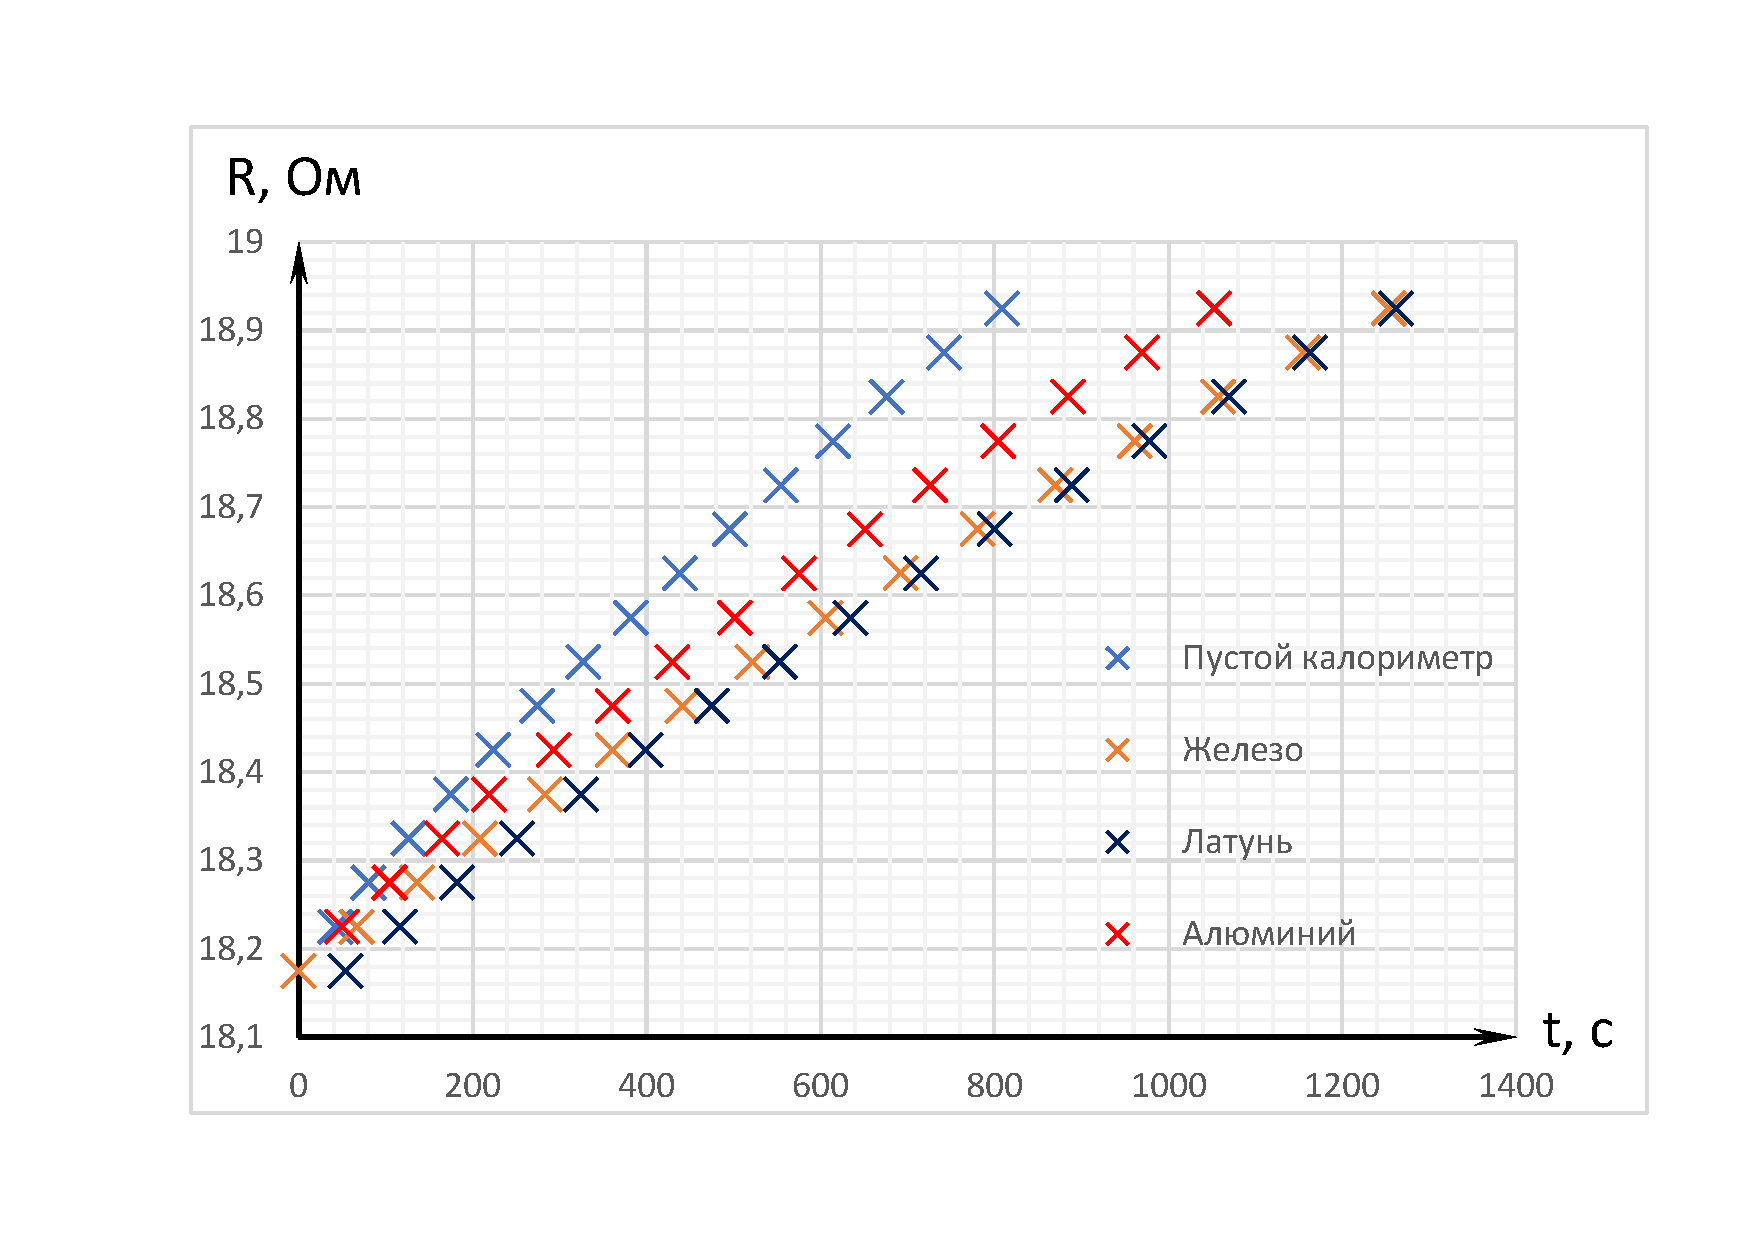
\includegraphics[width = \textwidth]{results_of_measuring}
			\caption{График зависимости сопротивления от времени нагрева}
			\label{fig:results_of_measuring}
		\end{center}
	\end{figure}
	
	По полученным данным построим также графики зависимостей $\frac{dR}{dt} \left( R \right)$ для различных серий измерений, т.е. для калориметра и 3 исследуемых образцов. Данную зависимость построим с учетом формулы:
	
	\begin{equation}
		\frac{dR}{dt} \left( R_{t_{1}} \right) = \frac{R_{t_{2}} - R_{t_{2}}}{t_{2} - t_{1}}
		\label{eq:derivates}
	\end{equation}

	Применив формулу (\ref{eq:derivates})  к данным таблицы (\ref{tab:results_of_measuring_of_depence_resistance_for_time}), построим графики искомых зависимостей. Графики  изображены на рисунках (\ref{ris:dR_dt(r)_for_calorimetr}) - (\ref{ris:dR_dt(r)_for_aluminium})
	
	\begin{figure}[h!]
		\begin{center}
			\begin{minipage}[h]{0.48\linewidth}
				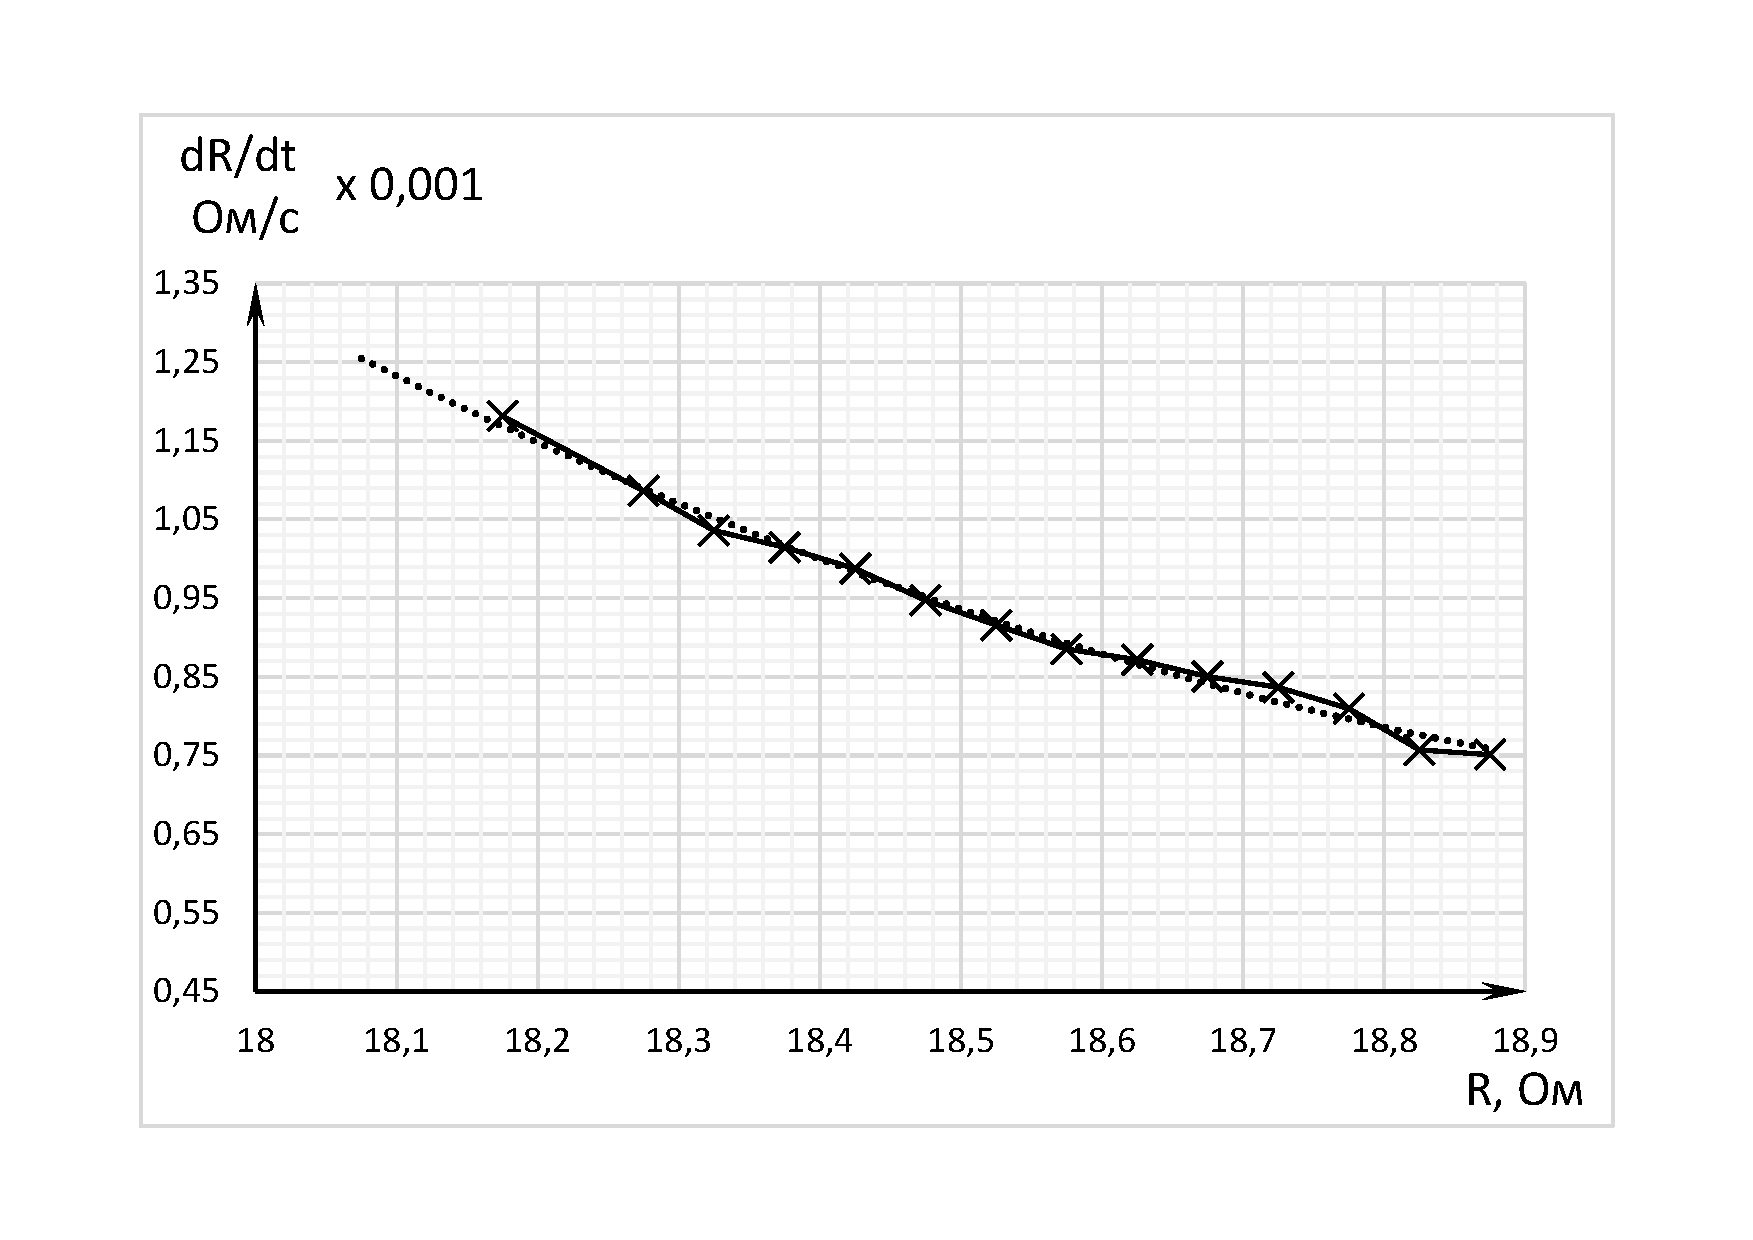
\includegraphics[width=1\linewidth]{dR_dt(r)_for_calorimetr}
				\caption{Зависимость $\frac{dR}{dt} \left( R \right)$ для калориметра} %% подпись к рисунку
				\label{ris:dR_dt(r)_for_calorimetr} %% метка рисунка для ссылки на него
			\end{minipage}
		\hfill
			\begin{minipage}[h]{0.48\linewidth}
				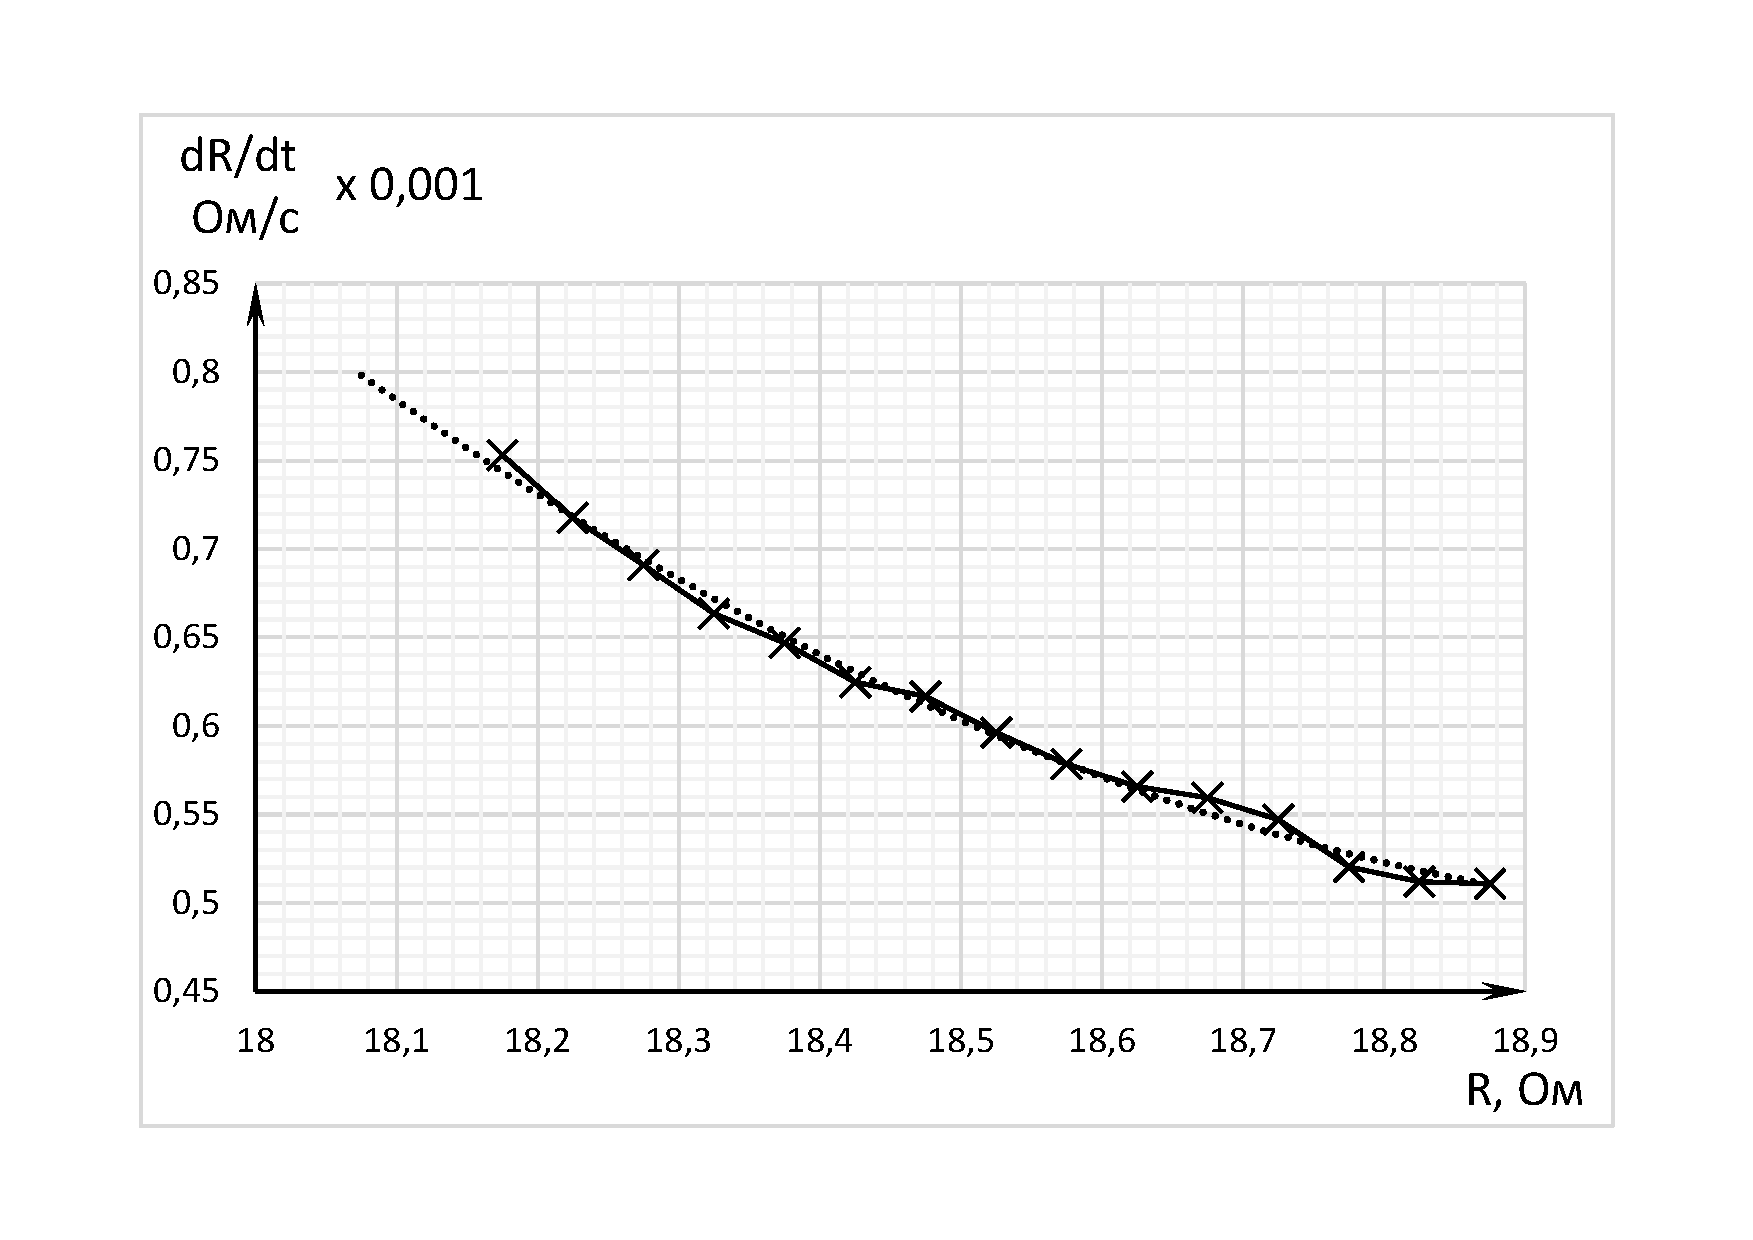
\includegraphics[width=1\linewidth]{dR_dt(r)_for_steel}
				\caption{Зависимость $\frac{dR}{dt} \left( R \right)$ для железного образца}
				\label{ris:dR_dt(r)_for_steel}
			\end{minipage}
		\end{center}
		\begin{center}
			\begin{minipage}[h]{0.48\linewidth}
				\includegraphics[width=1\linewidth]{dR_dt(r)_for_latun'}
				\caption{Зависимость $\frac{dR}{dt} \left( R \right)$ для латунного образца} 
				\label{ris:dR_dt(r)_for_latun'} %% метка рисунка для ссылки на него
			\end{minipage}
		\hfill
			\begin{minipage}[h]{0.48\linewidth}
				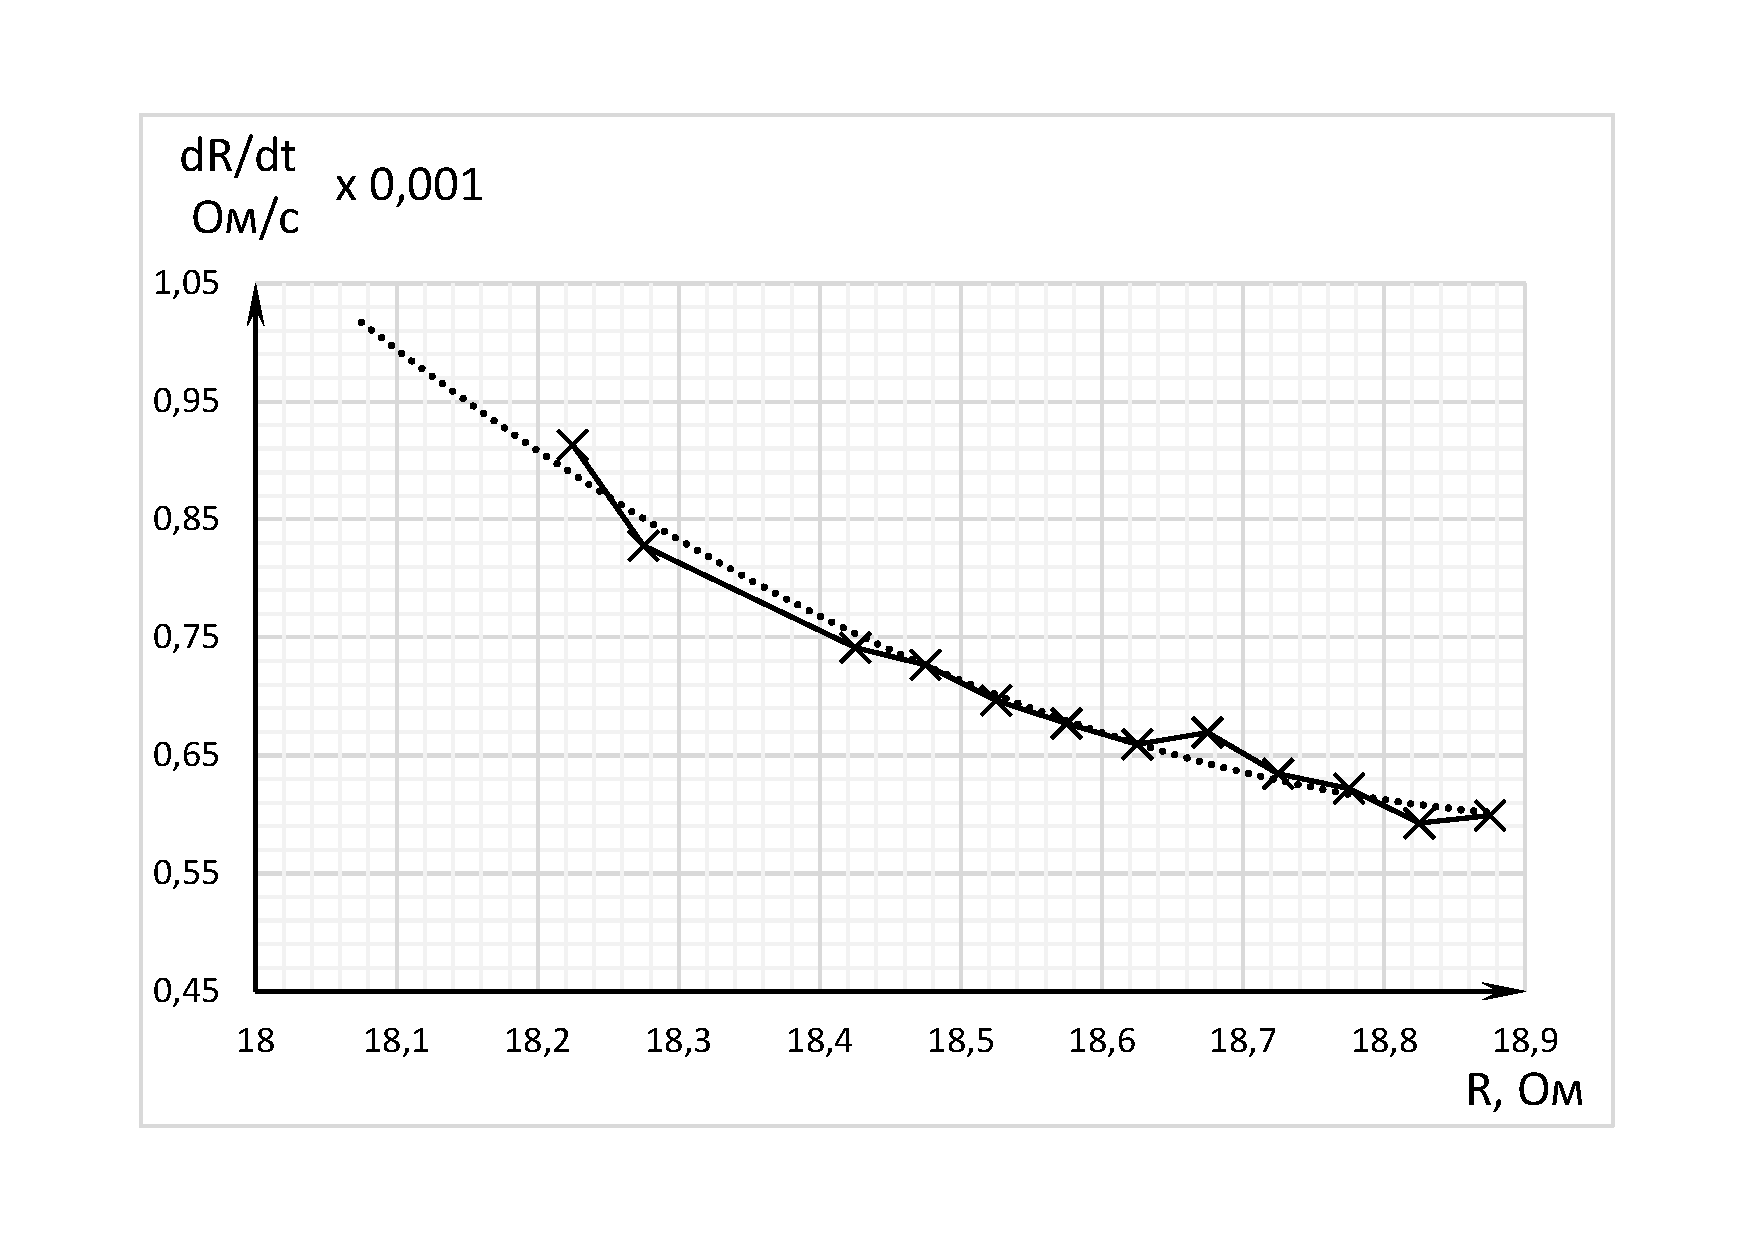
\includegraphics[width=1\linewidth]{dR_dt(r)_for_aluminium}
				\caption{Зависимость $\frac{dR}{dt} \left( R \right)$ для алюминиевого образца}
				\label{ris:dR_dt(r)_for_aluminium}
			\end{minipage}
		\end{center}
	\end{figure}
	
	Для экстраполяции зависимостей к значению $R_{T} = R_{K}$ применим полиномиальную аппроксимацию с показателем степени равным 2 (квадратичная аппроксимация).
	
	Тогда, для полученных зависимостей, после применения аппроксимации, получим  уравнения зависимости  (\ref{eq:derivates}), занесенные в таблицу (\ref{tab:extrapolation_results}).
	
	\begin{table}[h!]
		\centering
		\begin{tabular}{|c|c|}
		\hline
		исследуемое тело    & экстраполированное уравнение заисимости (7)                                                                                              		\\ \hline
		калориметр          & $\frac{dR}{dt} \left( R \right) = 0,000344R^{2} - 0,01336R + 0,13$     \\ \hline
		стальной образец    & $\frac{dR}{dt} \left( R \right) = 0,0002645R^{2} - 0,010134R + 0,0975$ \\ \hline
		латунный образец    & $\frac{dR}{dt} \left( R \right) = 0,000270R^{2} - 0,01037R + 0,1$      \\ \hline
		алюминиевый образец & $\frac{dR}{dt} \left( R \right) = 0,000520R^{2} - 0,01973R + 0,1878$   \\ \hline
		\end{tabular}
		\caption{Результаты экстраполяции зависимостей $\frac{dR}{dt} \left( R \right)$ для различных образцов}
		\label{tab:extrapolation_results}
	\end{table}
	
	Используя уравнения, приведенные в таблице (\ref{tab:extrapolation_results}), подставляя $R_{K} = 18,105 \, \text{Ом}$, определяем значения $\frac{dR}{dt} \left( R_{K} \right)$. Результаты занесем в таблицу (\ref{tab:derivates_results}).
	
	\begin{table}[h!]
		\centering
		\begin{tabular}{|c|c|}
		\hline
		исследуемое тело & $\frac{dR}{dt} \left( R_{K} \right)$, $\frac{\text{Ом}}{\text{с}} \cdot 10^{-4}$ \\ \hline
		калориметр          & 12,3 \\ \hline
		стальной образец    & 7,8  \\ \hline
		латунный образец    & 8,2  \\ \hline
		алюминиевый образец & 9,9  \\ \hline
		\end{tabular}
		\caption{Значения $\frac{dR}{dt} \left( R_{K} \right)$ для различных образцов}
		\label{tab:derivates_results}
	\end{table}
	
	Для определения теплоемкости, как видно из формулы (\ref{eq:capacity}), необходимо определить разность температур для каждого значения сопротивления. Очевидно, что разность температур не зависит от исследуемого материала для каждого значения сопротивления $R$. Тогда достаточно провести измерения для одной серии измерений. Зависимость разницы температур $\Delta T$ от $R$ задается следующей формулой:
	
	\begin{equation}
		\Delta T = \frac{R_{T} - R_{K}}{R_{K} \cdot \alpha}
	\end{equation}
	
	Результаты занесем в таблицы (\ref{tab:first_results_for_capacity}), (\ref{tab:first_results_for_capacity}).
	
	\begin{table}[h!]
		\centering
		\begin{tabular}{|c||c|c|c|c|c|c|c|c|}
		\hline
		R, Ом         & 18,175   & 18,225   & 18,275   & 18,325   & 18,375   & 18,425   & 18,475   & 18,525   \\ \hline
		$\Delta T$, К & 0,903349 & 1,548599 & 2,193848 & 2,839098 & 3,484348 & 4,129597 & 4,774847 & 5,420096 \\ \hline \hline
		R, Ом         & 18,575   & 18,625   & 18,675   & 18,725   & 18,775   & 18,825   & 18,875   & 18,925   \\ \hline
		$\Delta T$, К & 6,065346 & 6,710595 & 7,355845 & 8,001094 & 8,646344 & 9,291593 & 9,936843 & 10,58209 \\ \hline
		\end{tabular}
		\caption{Зависимость разницы температур от сопротивления термометра.}
		\label{tab:diffrence_between_temperature}
	\end{table}
	
	Теперь, определив все величины, входящие в формулу (\ref{eq:capacity}), перейдем к вычислению теплоемкостей исследуемых образцов. Результаты вычислений занесем в таблицу
	
	\begin{table}[h!]
		\centering
		\begin{tabular}{|c|c|}
		\hline
		исследуемое тело                 & $C, \frac{\text{Дж}}{\text{К}}$  \\ \hline
		калориметр                       & 681 \\ \hline	
		калориметр + железный образец    & 1071 \\ \hline
		калориметр + латунный образец    & 1017 \\ \hline
		калориметр + алюминиевый образец & 846 \\ \hline
		\end{tabular}
		\caption{Результаты вычисления теплоемкостей}
		\label{tab:first_results_for_capacity}
	\end{table}
	
	\begin{table}[h!]
		\centering
		\begin{tabular}{|c|c|}
		\hline
		исследуемое тело                 & $C, \frac{\text{Дж}}{\text{К}}/, $  \\ \hline
		калориметр                       & 681 \\ \hline	
		железный образец  			     & 390 \\ \hline
		латунный образец   				 & 336 \\ \hline
		алюминиевый образец 			 & 164 \\ \hline
		\end{tabular}
		\caption{Результаты вычисления теплоемкостей}
		\label{tab:second_results_for_capacity}
	\end{table}
		
	Дополнительно определим удельную -- $c$  теплоемкость. Результаты занесем в таблицу (\ref{tab:ud_capacity})
	
	\begin{table}[h!]
		\centering
		\begin{tabular}{|c|c|}
		\hline
		исследуемый образец & $c, \frac{\text{Дж}}{\text{кг К}}$ \\ \hline
		железный образец    & 478                           \\ \hline
		латунный образец    & 383                           \\ \hline
		алюминиевый образец & 572                           \\ \hline
		\end{tabular}
		\caption{Удельные теплоемкости для образцов}
		\label{tab:ud_capacity}
	\end{table}	
	
	\section{Определение погрешностей}
	
	Для определения погрешностей косвенных измерений, учтем, что погрешность измерения сопротивления $\sigma_{R}$ крайне мала, так как используется довольно точный метод с использованием Моста.
	
	Основной вклад в погрешность итоговых значений (теплоемкость, удельная теплоемкость) внесла погрешность экстраполяции функции, необходимая для определения коэффициента в итоговой функции.
	
	Поскольку данная ошибка гораздо больше чем погрешности прямых измерений, то для итогового расчета можно использовать только ее.
	
	\newpage
	
	$$\varepsilon_{\text{экстраполяции, калориметр}} = 0,11,\quad \varepsilon_{\text{экстраполяции, железный образец}} = 0,056$$
	
	$$\varepsilon_{\text{экстраполяции, латунный образец}} = 0,059, \quad \varepsilon_{\text{экстраполяции, алюминиевый образец}} = 0,094$$
	
	Определяя погрешности итоговых значений, получаем:
	
	Для теплоемкости:
	
	$$\sigma_{C, \text{калориметр}} = 68\frac{\text{Дж}}{\text{К}}, \quad \sigma_{C, \text{железный образец}} = 15\frac{\text{Дж}}{\text{К}}$$
	
	$$\sigma_{C, \text{латунный образец}} = 12\frac{\text{Дж}}{\text{К}}, \quad \sigma_{C, \text{алюминиевый образец}} = 17\frac{\text{Дж}}{\text{К}}$$
	
	Для удельной теплоемкости:
	
	$$\sigma_{c, \text{железный образец}} = 10\frac{\text{Дж}}{\text{кг К}}, \quad \sigma_{c, \text{латунный образец}} = 8\frac{\text{Дж}}{\text{кг К}}$$
	
	$$\sigma_{c, \text{алюминиевый образец}} = 59\frac{\text{Дж}}{\text{кг К}}$$
	
	Итоговые значения определенных величин:
	
	\begin{table}[h!]
		\centering
		\begin{tabular}{|c|c|c|}
		\hline
		исследуемое тело & $C, \frac{\text{Дж}}{\text{К}}$ & $c, \frac{\text{Дж}}{\text{кг К}}$ \\ \hline
		калориметр          & $681 \pm 68 $ & --            \\ \hline
		железный образец    & $389 \pm 15 $ & $478 \pm 10 $ \\ \hline
		латунный образец    & $335 \pm 12 $ & $383 \pm 8 $  \\ \hline
		алюминиевый образец & $167 \pm 17 $ & $572 \pm 59 $ \\ \hline
		\end{tabular}
		\caption{Итоговые значения определяемых величин.}
		\label{tab:final_tab}
	\end{table}
		
	\newpage
	
\section{Выводы}

\begin{enumerate}

	\item  Полученные значения удельных теплоемкостей для железа и латунь хорошо согласуются с табличными данными -- $480 \frac{\text{Дж}}{\text{кг  К}}$ и $478 \pm 10 \frac{\text{Дж}}{\text{кг  К}}$; $380 \frac{\text{Дж}}{\text{кг  К}}$ и $383 \pm 8 \frac{\text{Дж}}{\text{кг  К}}$. Для алюминия табличное значение полностью не соответствует определенному в ходе работы -- $920 \frac{\text{Дж}}{\text{кг  К}}$  и $572 \pm 59 \frac{\text{Дж}}{\text{кг  К}}$.
	
	\item Основной вклад в погрешности итоговых значений внесли: экстраполяция зависимости по графику функции и  промахи в измерении время нагрева до определенной температуры (Промахи касаются только калориметра и алюминиевого образца). 
	
	\item Достигнута приемлемая предельная точность -- $max \, \varepsilon = 0,11$.
	
	\item Экспериментально подтверждена правильность и работоспособность выбранной методики определения теплоемкости для твердых тел.
	
\end{enumerate}


\end{document}
